\newcommand{\op}{{\texttt{op}}}
\newcommand{\addr}{{\texttt{addr}}}
\newcommand{\data}{{\texttt{data}}}

To motivate Oblivious RAM, let us think of Signal's usage scenario.
Signal is an encrypted messenger app with billions of users. They want
to support a private contact discovery application. In contact
discovery, a user Alice sends her address book to Signal, and Signal
will look up its user database and return Alice the information about
her friends. The problem is that many users want to keep their address
book private, and Signal wants to provide contact discovery without
learning the users' contacts.

A naive solution is to rely on trusted hardware. Suppose Signal has a
secure processor (like Intel SGX) on its server. One can think of the
secure processor as providing a hardware sandbox (often referred to as
an \emph{enclave}). Now, Alice sends her address book in encrypted
format to the server's enclave; further, the server's database is also
encrypted as it is stored in memory and on disk. Now, the enclave has a
secret key that can decrypt the data and perform computation inside. At
first sight, this seems to solve the privacy problem, since data is
always encrypted in transit and at rest, and the server cannot see the
contents.

Unfortunately, encryption alone provides little privacy in such
scenarios. The enclave will need to access encrypted entries stored on
disk, and the server's operating system can easily observe the
\emph{access patterns}, i.e., which memory pages are being fetched by
the enclave. The access patterns leak exactly who Alice's friends are
even if the data is encrypted!

In general, access patterns of a program leak sensitive information
about your private data. As a simpler example, if you are performing
binary search over a sorted array, the entries accessed during the
search would leak your private query.

We can also think of access pattern leakage through a programming
language perspective. For example, the following program has an
\texttt{if}-branch dependent on secret inputs. (Maybe the secret input
is the last bit of a secret key). By observing whether memory location
\texttt{x} or \texttt{y} is accessed, one can infer which branch is
taken.

\begin{center}
\begin{minipage}{22mm}
\begin{verbatim}
if (s) {
  mem[x]
} else {
  mem[y]
}
\end{verbatim}
\end{minipage}
\end{center}

Therefore, we want to solve the following challenge:

\begin{quote}
{\it How can we provably hide access patterns while preserving efficiency?}
\end{quote}

The solution Signal eventually deployed is an algorithmic technique
called Oblivious RAM (ORAM).

\subsection{Oblivious RAM: problem
definitions}
\label{oblivious-ram-problem-definitions}

Oblivious RAM (ORAM) is a powerful cryptographic protocol that
\emph{provably} hides access patterns to sensitive data.

We would like to ensure a very strong notion of security. In particular,
no information should be leaked about: 1) which data block is being
accessed; 2) the age of the data block (when it was last accessed); 3)
whether a single block is being requested repeatedly (frequency); 4)
whether data blocks are often being accessed together (co-occurrence);
or 5) whether each access is a read or a write.

Let us explain the parts of an ORAM system.

An ORAM algorithm (the \emph{client}) sits between a \emph{user} who
wants to access memory and a \emph{server} that has memory capabilities.
At the server-ORAM interface, the server simply acts as a memory: The
ORAM client sends read and write requests to the server, and the server
responds. Between the ORAM and the user, the user submits \emph{logical}
read and write requests to the ORAM client, and the client will reply to
each (after interaction with the server).

We will call \emph{physical} memory the memory that the server manages,
and \emph{logical} memory the memory the user wants to access. Memory,
both physical and logical, will be made up of ``blocks''; our ORAM
algorithm will support \(N\) blocks of logical memory.

Formally, the user sends to the algorithm a sequence of \emph{logical}
requests, where each logical request is of the form
\((\texttt{read},\texttt{addr})\) or
\((\texttt{write}, \texttt{addr}, \texttt{data})\).

After each user request, the ORAM algorithm interacts with the server to
make a sequence of \emph{physical} memory accesses, where each physical
access either reads or writes a block to a physical location.

And finally, the ORAM algorithm turns back to the user and returns an
answer to the logical request.

For example, in Signal's scenario, the ``user'' and the ``ORAM client''
are both in the hardware enclave, and the ``ORAM server'' is the
untrusted memory and disk on Signal's server.

The security requirement for ORAM is that the server should learn
nothing about the user's logical memory requests from observing the
sequence of physical memory requests. For any two \emph{logical} request
sequences, the ORAM's resulting \emph{physical} access sequences will be
indistinguishable.

\begin{remark}
In this security requirement, we require that the server learn nothing
from observing only the list of physical addresses, and whether each
physical access is a read or write. We do not say anything about the
data that is written to physical memory.

In practice, we need to use encryption to hide the contents of the
blocks. If we read a block and then write it back, we should re-encrypt
it with a different ciphertext, or else the server would recognize it as
the same block.

From now on we will simply assume secure encryption as given, and focus
on hiding the access patterns.
\end{remark}

\subsection{Naive solutions}\label{naive-solutions}

\subsubsection{Naive solution 1}\label{naive-solution-1.}

One trivial solution is for the client to read all blocks from the
server upon every logical request. Obviously this scheme leaks nothing
but would be prohibitively expensive.

\subsubsection{Naive solution 2}\label{naive-solution-2.}

Another trivial solution is for the client to store all blocks, and thus
the client need not access the server to answer any memory request. But
this defeats the numerous advantages of cloud outsourcing in the first
place. \emph{Henceforth, we require that client store only a small
amount of blocks} (maybe constant or polylogarithmic in \(N\)).

\subsubsection{Naive solution 3}\label{naive-solution-3.}

Another naive idea is to randomly permute all memory blocks through a
secret permutation known only to the client. Whenever the client wishes
to access a block, it will appear to the server to reside at a random
location.

Indeed, this scheme gives a secure \emph{one-time} ORAM scheme: It
provides security if every block is accessed only once. However, if the
client needs to access each block multiple times, then the access
patterns will leak statistical information such as frequency (how often
the same block is accessed) and co-occurrence (how likely two blocks are
accessed together). As mentioned earlier, one can leverage\footnote{https://www.ndss-symposium.org/wp-content/uploads/2017/09/06\_1.pdf}
such statistical information to infer sensitive secrets.

\subsubsection{Important observation}\label{important-observation.}

The above naive solution 3 gives us the following useful insight:
Informally, if we want a ``non-trivial'' ORAM scheme, it appears that we
may have to relocate a block after it is accessed --- otherwise, if the
next access to the same block goes back to the same location, we can
thus leak statistical information. It helps to keep this observation in
mind when we describe our ORAM scheme later.

\subsection{Binary-tree ORAM: data structure}\label{data-structure}

We will learn about tree-based ORAMs. Then, we will mention an
improvement called Path ORAM,\footnote{https://eprint.iacr.org/2013/280.pdf}
which is the scheme that Signal has deployed.

\subsubsection{Server data structure}\label{server-data-structure.}

The server stores a binary tree with \(N\) leaves. (If necessary,
replace \(N\) with the next larger power of \(2\).)

Each node is called a \emph{bucket}, and each bucket is a finite array
that can hold up to \(Z\) number of blocks --- for now, think of \(Z\)
as being relatively small (maybe polylogarithmic in \(N\)); we will
describe how to parametrize \(Z\) later. Some of the blocks stored by
the server are \emph{real}; other blocks are \emph{dummy}. As will be
clear later, these dummy blocks are introduced for security: We do not
want the server to learn which buckets hold real blocks.

\subsubsection{Main path invariant}\label{main-path-invariant.}

The most important invariant is that at any point of time, each block is
mapped to a random path in the tree (also referred to as the block's
designated path), where a path begins from the root and ends at some
leaf node --- and thus a path can be specified by the corresponding leaf
node's identifier. When a block is mapped to a path, it means that the
block can legitimately reside anywhere along the path.

\subsubsection{Imaginary position map}\label{imaginary-position-map.}

For the time being, we will rely on the following cheat (an assumption
that we can get rid of later). We assume that the client can store a
somewhat large position map that records the designated path of every
block. In general, such a position map would require roughly
\(\Theta( N\log N )\) bits to store --- but later we can
recursively outsource the storage of the position map to the server by
placing position maps in progressively smaller ORAMs.

\subsection{Binary-tree ORAM: operations}\label{operations}

We now describe how to access blocks in our ORAM scheme.

\subsubsection{Fetching a block}\label{fetching-a-block.}

Given how our data structures are set up, accessing a block is very
easy: the client simply looks up its local position map, finds out on
which path the block is residing, and then reads each and every block on
the path. As long as the main invariant is respected, the client is
guaranteed to find the desired block.

\subsubsection{Remapping a block}\label{remapping-a-block.}

Recall that earlier, we have gained the informal insight that whenever a
block is accessed, it should relocate. Here, whenever we access a block,
we must remap it to a randomly chosen new path --- otherwise, we would
end up going back to the same path if the block is requested again, thus
leaking statistical information.

To remap the block, we choose a fresh new path, and we update the
client's position map to associate the new path with the block. We now
would like to write this block back to the tree, to somewhere on the new
path (and if the request is a \texttt{write} request, the block's
contents are updated before being written back to the server). But doing
this is tricky! It turns out that we cannot write the block back
directly to the leaf bucket of the new path, since doing so would reveal
which new path the block got assigned to. For the same reason, we cannot
write this block back to any internal nodes of the new path either,
since writing to any internal node on the new path also leaks partial
information about the new path.

It turns out that the only safe location to write the block back is to
the root bucket! The root bucket resides on every path, and thus writing
the block back to the root does not violate the main path invariant; and
further, it does not leak any information about the new path.

Now this is great. Our idea thus is to write this block back to the root
bucket. However, there is also an obvious problem. The root bucket has a
capacity of \(Z\), and if we keep writing blocks back to the root, soon
enough the root bucket will overflow! Therefore, we now introduce a new
procedure called \emph{eviction} to cope with this problem.

\subsubsection{Eviction}\label{eviction.}

Eviction is a maintenance operation performed upon every data access to
ensure that none of the buckets in the ORAM tree will ever overflow
except with negligible in \(N\) failure probability. Note that if an
overflow does happen, the block that leads to the overflow can get lost
since there is no space to hold it on the server, and this can affect
the correctness of our ORAM scheme. However, we will guarantee that such
correctness failure happens only with negligible probability.

The high-level idea is very simple: Whenever we can, we will try to move
blocks in the tree closer to the leaves, to allow space to free up in
smaller levels of the tree (levels closer to the root). There are a few
important considerations when performing such eviction:

\begin{itemize}
\item
  Data movement during eviction must respect the main path invariant:
  Each block can only be moved into buckets in which it can legitimately
  reside.
\item
  Data movement during eviction must retain \emph{obliviousness}: The
  physical locations accessed during eviction should be independent of
  the input requests to the ORAM.
\item
  As we perform eviction, we pay a cost for this maintenance operation
  and the cost is charged to each data access. Obviously, if we are
  willing to pay more such cost, we can pack blocks closer to the
  leaves, thus leaving more room in smaller levels. In this way,
  overflows are less likely to happen. On the other hand, we also do not
  want the eviction cost to be too expensive. Therefore, another tricky
  issue is how we can design an eviction algorithm that achieves the
  best of both worlds: With a small number of eviction operations, we
  want to keep the probability of overflow very small (technically:
  negligible in \(N\)).
\end{itemize}

\begin{figure}[t]
\centering
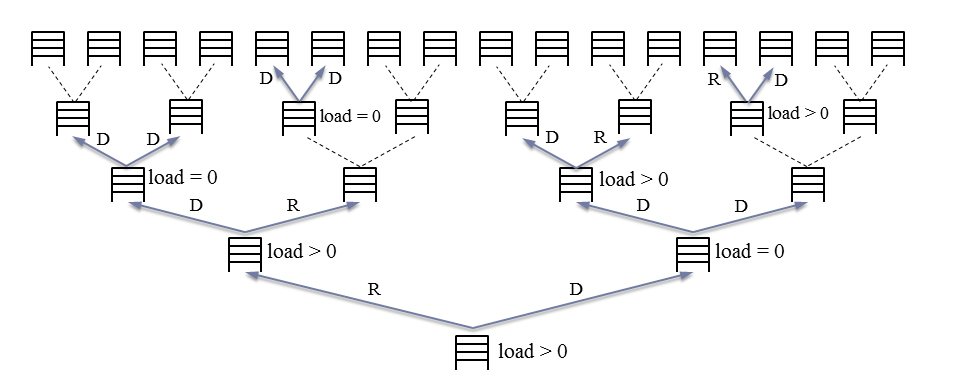
\includegraphics[width=\textwidth]{binaryoram16-evict.png}
\caption{The \texttt{Evict} algorithm. Upon every data access operation,
two buckets are chosen at every level of the tree for eviction during
which one data block will be evicted to one of its children. To ensure
security, a dummy eviction is performed for the child that does not
receive a block; further, if the bucket chosen for eviction is empty,
dummy evictions are performed on both child buckets. In this figure,
\(R\) denotes a real eviction and \(D\) denotes a dummy eviction.}
\end{figure}

We describe a simple candidate eviction scheme, and we will give an
informal analysis of the scheme later:

\begin{itemize}
\item
  \emph{{[}An eviction algorithm{]}} Upon every data access, we choose
  at random \(2\) buckets in every level of the tree for eviction (for
  the root level, pick one bucket). If a bucket is chosen for eviction,
  we will pop an arbitrary block (if one exists) from the bucket, and
  write the block to one of its children.
\end{itemize}

Note that depending on the chosen block's designated path, there is only
one child where the block can legitimately go. We must take precautions
to hide where this block is going: Thus for the remaining child that
does not receive a block, we can perform a ``dummy'' eviction.
Additionally, if the bucket chosen for eviction is empty (does not
contain any real blocks), then we make a dummy eviction for both
children --- this way we avoid leaking the information that the chosen
bucket is empty.

More specifically, to write an intended block to a child bucket, we
sequentially scan through the child bucket. If the slot is occupied with
a real block, we simply write the block back. If the slot is empty, we
write the intended block into that slot. A dummy eviction therefore is
basically reading every block sequentially and writing the original
contents back.

So far, we have not argued why any bucket that receives a block always
has space for this block --- we will give an informal analysis later to
show that this is indeed the case.

\subsubsection{Algorithm pseudo-code}\label{algorithm-pseudo-code.}

We present the algorithm's pseudo-code in Algorithms~\ref{alg:access}
and \ref{alg:evict}.

\begin{algo}{$\texttt{The procedure Access}(\texttt{op}, \texttt{addr}, \texttt{data}^*)$ where $\texttt{op} = \texttt{read}$ or $\texttt{op} = \texttt{write}$}
\label{alg:access}

\textbf{Assume:}
Each block is of the form $(\addr, \data, l)$
where $l$ denotes the block's current designated path.

%\begin{figure*}[t]
\begin{algorithmic}[1]
%\REQUIRE Logical address requested block $\addr$. The client's position map $\texttt{position}$.
%\ENSURE $l^{*}$ as the new path identifier of the requested block. 
%$\texttt{data}$ as the data fetched.
\STATE Let $l^{*}$ be a random value from $1$ to $N$.
%\texttt{UniformRandom}(\{0, 1\} ^ D)$.
Assign $l \leftarrow \texttt{position}[\addr]$, $\texttt{position}[\addr] \leftarrow l^{*}$.
\FOR{each $\textsf{bucket}$ from leaf $l$ to root}
	\STATE Scan $\textsf{bucket}$, and if  
$(\addr, \data_0, \_) \in \textsf{bucket}$ then 
let $\textsf{data}^* \leftarrow \textsf{data}_0$ and 
remove this block from \textsf{bucket}.
%    \IF{$(\addr, \data_0, \_) \in \textsf{B}$}
        %\STATE $\texttt{data} \leftarrow \texttt{data}_0$.
%    \ENDIF
%    \STATE Rewrite the bucket $l_0$.
\ENDFOR

\STATE if $\op = \texttt{read}$ then add $(\addr, \data^*, l^*)$ to the root bucket;
else add $(\addr, \data, l^*)$ to the root bucket.

\STATE Call the $\texttt{Evict}$ subroutine.

\RETURN $\data^*$.

\end{algorithmic}
\end{algo}

\begin{algo}{The procedure \texttt{Evict}}
\label{alg:evict}
\begin{algorithmic}[1]
%\REQUIRE $\nu$ as the number of blocks to evict in each level.

\FOR{each level $d$ from root to the level of leaves $- 1$}
\STATE $\textsf{bucket}_0$, $\textsf{bucket}_1 \leftarrow$ 
randomly choose $2$ distinct buckets in the level $d$
(for the root level, pick one bucket).
\FOR{$\textsf{bucket}$ $\in$ $\{\textsf{bucket}_0, \textsf{bucket}_1\}$}
\STATE 
$\textsf{block} :=$ pop a real block from $\textsf{bucket}$
if one exists; else $\textsf{block} := (\bot, \bot, \bot)$.
%pop block $(\addr, \data, l)$ from $\textsf{bucket}$.
\STATE {for each of the two children of $\textsf{bucket}$ in a fixed order}:
scan the child bucket reading 
and writing every block. 
If $\textsf{block}$ is real and wants to go to  
the child, write $\textsf{block}$  to an empty slot in the child bucket.
%\ENDFOR
\ENDFOR
\ENDFOR
\end{algorithmic}
\end{algo}

\begin{remark}
Note that in a full-fledged implementation, 
all blocks are typically encrypted to hide the contents of the block.
Whenever reading and writing back a block, the block
must be re-encrypted prior to being written back.
If the encryption scheme is secure, the server should not be able
to tell whether the block's content has changed 
upon seeing the new ciphertext.
\end{remark}

\subsection{Analysis}\label{analysis}

We will now discuss why the aforementioned binary-tree ORAM construction

1) preserves obliviousness, and

2) is correct (except with negligible probability).

\subsubsection{Obliviousness}\label{obliviousness.}

Obliviousness is easy to see.
First, whenever a block is accessed, it is assigned to a new path and
the choice of the new path is kept secret from the server. So whenever
the block is accessed again, the server simply sees a random path being
accessed.
Second, the entire eviction process does not depend on the input
requests at all.

\subsubsection{Correctness}\label{correctness.}

Correctness is somewhat trickier to argue. As mentioned earlier, to
argue correctness, we must argue why no overflow will ever occur except
with negligible probability --- as long as the bucket size \(Z\) is set
appropriately.

strong(Claim):\\
\phantomsection\label{clm:bucketsize}{}

strong(Proof):\\
The full proof uses results from queueing theory,\footnote{https://en.wikipedia.org/wiki/Queueing\_theory}
in particular Burke\textquotesingle s theorem.\footnote{https://en.wikipedia.org/wiki/Burke\%27s\_theorem}
We will give a heuristic argument that does not require any specialized
knowledge.

\begin{itemize}
\item
  The root bucket (level \(0\) of the ORAM tree) receives exactly \(1\)
  incoming block with every access, and it is evicted on every access,
  so the root bucket always ends up empty.
\item
  There are \(N\) leaf buckets, and \(N\) blocks are assigned to them at
  random. We leave it as an exercise to check that the probability that
  more than \(( \log N )^{2}\) blocks are assigned to any one
  leaf is negligible than \(N\) (in other words: decays faster than
  \(N^{k}\), for every \(k\)).
\item
  Now consider a bucket, neither root nor leaf, at level \(i \geq 1\) of
  the ORAM tree. A block will enqueue on one out of every \(2^{i}\)
  accesses, and with probability \(\frac{1}{2^{i - 1}}\), the bucket is
  chosen for eviction.
\end{itemize}

So for every non-leaf and non-root level of the tree, with every ORAM
access, the dequeue probability is twice as large as the enqueue
probability. This situation is well-known in queueing theory as the
``M/M/1 queue'':

\begin{itemize}
\item
  Every time step, with probability \(p\), an item enqueues;
\item
  Every time step, with probability \(2p\), an item dequeues if the
  queue is non-empty.
\end{itemize}

Since the bucket is drained (on average) twice as fast as it is filled,
we expect that it is very unlikely for a lot of blocks to accumulate in
any one bucket.

Indeed, one can prove an exponential bound on the probability that any
one bucket gets too full:
\[\Pr [\mathrm{\text{number of items in queue}} > R] \leq \exp( \Omega( - R) ).\]

Unfortunately, this does not quite finish our analysis of the ORAM tree.
The reason is that the buckets in the ORAM tree are not independent, and
our informal argument above ignored possible dependence between buckets.
It turns out that this gap can be filled using Burke's theorem. But at
this point the reader should already be convinced that the result is at
least quite plausible.

\subsection{Binary-tree ORAM: recursion}\label{binary-tree-oram-recursion}

So far, we have cheated and pretended that the client can store a large
position map. We now describe how to get rid of this position map. The
idea is simple: Instead of storing the position map on the client side,
we simply store it in a smaller ORAM denoted
\(\mathsf{\text{posORAM}}_{1}\) on the server. The position map of
\(\mathsf{\text{posORAM}}_{1}\) will then be stored in an even smaller
ORAM denoted \(\mathsf{\text{posORAM}}_{2}\) on the server, and so on.
As long as the block size is at least \(\Omega( \log N )\)
bits, every time we recurse, the ORAM's size reduces by a constant
factor; and thus \(O( \log N )\) levels of recursion would
suffice.

We can thus conclude with the following theorem.

strong(Theorem):\\
Binary-tree ORAM\footnote{https://eprint.iacr.org/2011/407.pdf}: For any
super-constant function \(\alpha( \cdot )\), there is an ORAM scheme
that achieves \(O( \alpha\log^{3}N )\) cost for each access:
each logical request will translate to
\(O( \alpha\log^{3}N )\) physical accesses; and moreover, the
client is required to store only \(O(1)\) number of blocks.

Note that in the total cost \(O( \alpha\log^{3}N )\), an
\(\alpha\log N\) factor comes from the bucket size; another \(\log N\)
factor comes from the total height of the tree; and the remaining
\(\log N\) factors comes from the recursion.

\subsection{Path ORAM}\label{path-oram}

The design of the above binary-tree ORAM is a little silly: Whenever we
visit a triplet of buckets for eviction, we only evict one block. For
this reason, the bucket size needs to be super-logarithmic to get
negligible failure probability. It turns out that if we instead use a
more aggressive eviction algorithm, and with a more sophisticated proof,
the bucket size can be made constant. At this point, we are ready to
introduce an improved version called Path ORAM.

Unlike the above binary-tree ORAM, in Path ORAM, every bucket has
constant size (maybe 4 or 5), except the root bucket which is
super-logarithmic in size. Every time we access some path to fetch a
block, we also perform eviction on the same path. In particular, we will
rearrange the blocks on the path in the most aggressive manner possible:
We want to move the blocks as close to the leaf level as possible, but
\emph{without violating the path invariant}. With Path ORAM, every
access operation touches a single path, hence the name Path ORAM. The
cost of each access is \(O( \alpha\log^{2}N )\) for an
arbitarily small superconstant function \(\alpha\).

\subsubsection{Other applications of
ORAM}\label{other-applications-of-oram}

ORAM promises many potential applications. For instance, in Large
Language Models (LLMs), a commonly used technique is called Retrieval
Augmented Generation (RAG). RAG parses the user's query and looks up the
relevant locations in a large knowledge base to fetch the relevant
entries. If we want to protect the privacy of users' queries in LLMs, it
is also crucial to hide the access patterns, and this would be a great
application of ORAM.

Besides its usage in secure processors, ORAM is critical for scaling
cryptographic multi-party computation (MPC) to big data. Traditional MPC
techniques require us to express the desired computation as a circuit.
However, in the real-world, we program assuming the Random Access
Machine (RAM) model where a CPU can dynamically read and write a memory
array. Translating a RAM program to a circuit brute-force would incur a
linear (in the memory size) cost for each memory access! For example, a
binary search in a sorted database requires only logarithmic time on a
RAM, but it requires linear cost when expressed as a circuit.
Fortunately, ORAM again comes to our rescue. There is a line of work on
RAM-model MPC, and the idea is that we first translate the RAM to an
Oblivious RAM, and at this point all the memory accesses are safe to
reveal. At this moment, we can use MPC to securely emulate a ``secure
processor'' that performs computation while accessing memory
obliviously.
